\chapter{Method: DCT-Page}\label{chap:method}

DCT-Page modifies only the \emph{decode} path of attention.
During prefill the model runs unchanged, producing an ordinary
key--value (KV) cache.  At decode time the cache is reinterpreted as a
sequence of fixed-size pages, each page is summarized by a short
low-frequency proxy, and the query attends to a constant-size subset:
the sink, the top-$k$ pages by proxy score, and a small recent window.
The remaining pages are skipped entirely.
This chapter describes the layout, the proxy, the selection rule, and
the fused kernels that turn the resulting sparsity into measured
throughput.


\section{Decode-Time Page Layout}\label{sec:layout}

Let $L$ denote the current KV-cache length and $P$ the page size
(default $P{=}32$).  Let $S$ and $R$ be the number of sink and full
recent pages, respectively.  The cache is partitioned as
\begin{equation}\label{eq:layout}
  \underbrace{[\,0,\; SP\,)}_{\text{sink}}\;\Big\|\;
  \underbrace{[\,SP,\; SP{+}NP\,)}_{\text{middle pages}}\;\Big\|\;
  \underbrace{[\,SP{+}NP,\; L\,)}_{\text{recent}},
\end{equation}
where
\begin{equation}\label{eq:num-pages}
  N \;=\; \left\lfloor \frac{L - SP - RP}{P} \right\rfloor
\end{equation}
is the number of \emph{middle} pages, i.e.\ the pageable region from
which DCT-Page selects.
The recent zone consists of $R$ full pages plus a partial \emph{open}
page that absorbs the most recent $0,\dots,P{-}1$ tokens; the open page
is always attended in full.
Figure~\ref{fig:layout} shows the layout for $S{=}1,\ R{=}4$, the
defaults used throughout this thesis.

\begin{figure}[ht]
  \centering
  \begin{tikzpicture}[
    page/.style={draw, rectangle, minimum height=10mm, minimum width=10mm,
                 inner sep=0pt, font=\footnotesize},
    sink/.style ={page, fill=orange!25},
    mid/.style  ={page, fill=blue!12},
    selmid/.style={page, fill=blue!45},
    rec/.style  ={page, fill=green!25},
    open/.style ={page, fill=green!10, dashed},
    brace/.style={decoration={brace, amplitude=4pt, mirror}, decorate, thick},
    lbl/.style={font=\footnotesize}
  ]
    % Cells
    \node[sink]                     (s0)  at (0,0)        {$\mathrm{sink}$};
    \node[mid,    right=0mm of s0]  (m0)                  {$0$};
    \node[selmid, right=0mm of m0]  (m1)                  {$1$};
    \node[mid,    right=0mm of m1]  (m2)                  {$2$};
    \node[mid,    right=0mm of m2]  (m3)                  {$\cdots$};
    \node[selmid, right=0mm of m3]  (m4)                  {$N{-}2$};
    \node[mid,    right=0mm of m4]  (m5)                  {$N{-}1$};
    \node[rec,    right=0mm of m5]  (r0)                  {$r_0$};
    \node[rec,    right=0mm of r0]  (r1)                  {$\cdots$};
    \node[rec,    right=0mm of r1]  (r2)                  {$r_{R-1}$};
    \node[open,   right=0mm of r2]  (op)                  {open};

    % Braces and labels (mirror=true so the central peak points up toward
    % the cells; the labels sit below).
    \draw[brace] ($(s0.south west)+(0,-1mm)$)
              -- ($(s0.south east)+(0,-1mm)$)
       node[midway, below=6pt, lbl] {$S$ pages};
    \draw[brace] ($(m0.south west)+(0,-1mm)$)
              -- ($(m5.south east)+(0,-1mm)$)
       node[midway, below=6pt, lbl] {$N$ middle pages (selectable)};
    \draw[brace] ($(r0.south west)+(0,-1mm)$)
              -- ($(op.south east)+(0,-1mm)$)
       node[midway, below=6pt, lbl] {$R$ full + 1 open};

    % Top label
    \node[above=1mm of m3, lbl] {$\text{KV positions } 0,\dots,L-1$};
  \end{tikzpicture}
  \caption[Decode-time KV page layout used by DCT-Page.]
  {Decode-time KV layout. The sink and recent zones are always
  attended; only the $N$ middle pages enter the top-$k$ selection.
  Darker blue cells indicate two example selected pages.}
  \label{fig:layout}
\end{figure}

\paragraph{Sink and recent zones.}
The sink absorbs the initial-token attention sinks observed in
autoregressive decoder transformers and is kept verbatim to preserve
position-aware behaviors learned during pretraining.
The recent window protects the most local context, which dominates the
output for generation tasks and is cheap to keep at full resolution.

\paragraph{Page granularity.}
The page size is the fundamental trade-off knob.  A smaller $P$ gives
finer selection but raises bookkeeping cost (more pages, more scores,
more top-$k$ work).  A larger $P$ amortizes overhead but loses
selectivity within the page.  We use $P{=}32$ throughout, which is
also the granularity at which contemporary sparse-attention systems
operate (Quest, SeerAttention-R, Multipole).

\paragraph{Fallback below short context.}
When $L$ is short, the savings from sparsification are dominated by
the bookkeeping overhead of scoring and assembly.  DCT-Page therefore
falls back to standard dense decode attention when
$L < L_\text{min}$, with $L_\text{min}{=}8192$ tokens by default.


\section{Key Insight: Low-Frequency Structure of Attention Keys}\label{sec:insight}

The starting point for the rest of this chapter is a single empirical
observation about decoder-transformer key vectors: viewed as a signal
along the sequence axis, they are overwhelmingly low-frequency.

Concretely, take a page of $P{=}32$ consecutive keys
$K_p \in \mathbb{R}^{P \times d}$ from a single (batch, layer, head)
triple and apply the orthonormal type-II discrete cosine transform
along the sequence axis,
\begin{equation}\label{eq:dct}
  \hat K_p[m, c] \;=\;
  \sqrt{\tfrac{2}{P}}\, \alpha_m \sum_{n=0}^{P-1}
  K_p[n, c]\,
  \cos\!\left(\tfrac{\pi (2n{+}1) m}{2P}\right),
  \quad m = 0,\dots,P{-}1,
\end{equation}
with $\alpha_0 = 1/\sqrt{2}$ and $\alpha_m = 1$ for $m \ge 1$.
Here $\hat K_p \in \mathbb{R}^{P \times d}$ is the frequency-domain
representation of the page: row index $m$ runs over DCT bins from low
($m{=}0$, the DC term) to high frequency, and each column $c$ holds
the spectrum of one of the $d$ feature channels.
By Parseval's theorem (DCT is orthonormal), the total energy of $K_p$
equals the sum of squared coefficients $\sum_m \|\hat K_p[m, :]\|^2$.
On a RULER NIAH-MultiKey~3 trace at 32K context with
Llama-3.1-8B-Instruct, the first four DCT bins ($m = 0, 1, 2, 3$)
capture, on average, $\approx 85\%$ of the total per-page key energy
across layers, and the first eight bins reach $\approx 90\%$; the
remaining high-frequency tail contributes negligibly
(Figure~\ref{fig:dct-energy}).

\begin{figure}[ht]
  \centering
  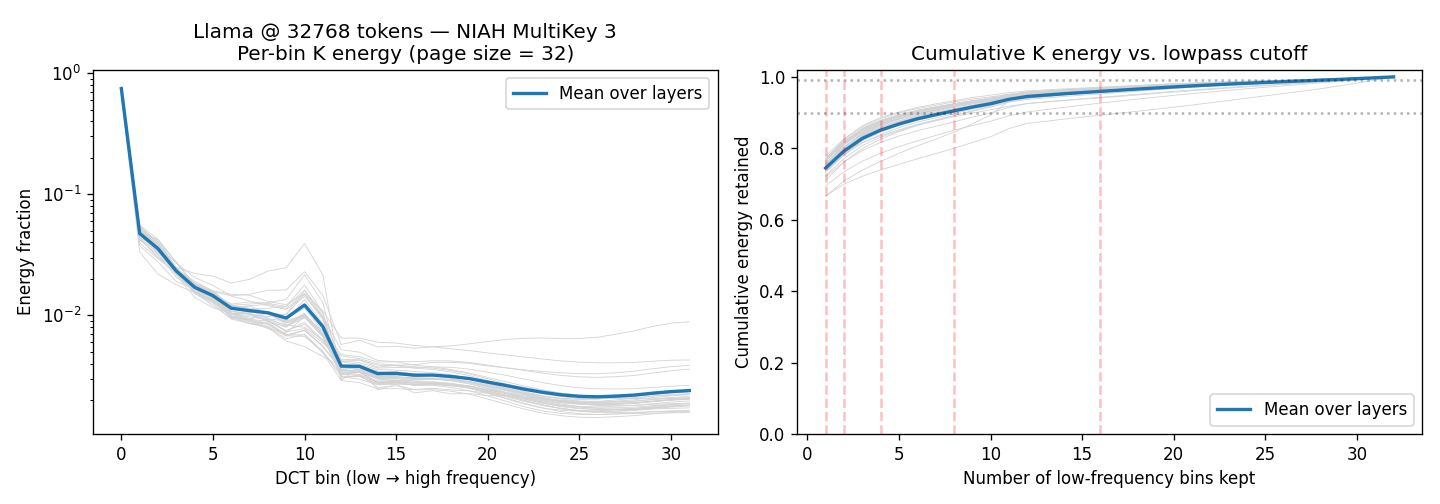
\includegraphics[width=0.95\textwidth]{figures/energy_curve.png}
  \caption[Per-bin DCT energy of KV-cache key pages.]
  {Per-bin DCT energy and cumulative energy of decoder-transformer
  key pages on Llama-3.1-8B-Instruct, page size $P{=}32$, RULER
  NIAH-MultiKey~3 at 32K context. Left: per-bin energy fraction;
  each thin grey line is a single transformer layer, the thick blue
  line is the across-layer mean. The spectrum is strongly low-pass.
  Right: cumulative fraction of energy retained as a function of the
  lowpass cutoff; the first four bins already cover $\approx 85\%$
  of the per-page energy and eight bins cover $\approx 90\%$.}
  \label{fig:dct-energy}
\end{figure}

This concentration has a direct consequence for sparse attention.
The attention score that determines whether page $p$ should be
selected for a query $q$ is the inner product
$q^\top K_p[n, \cdot]$ for some token $n$ in the page.  If $K_p$
itself lives in a low-rank low-frequency subspace, then a DCT-lowpass
reconstruction of $K_p$ should be a near-lossless proxy for the
selection score, even after collapsing $P$ tokens into a handful of
representative tokens.  The next section formalizes this proxy and
quantifies how well it routes queries to the right page.


\section{DCT-lowpass-IDCT Page Proxy}\label{sec:proxy}

Section~\ref{sec:insight} established that a page of keys
$K_p \in \mathbb{R}^{P \times d}$ is concentrated in its leading DCT
bins.  DCT-Page exploits this by replacing each page with a much
shorter sequence that retains only those bins.

Fix a target proxy length $C$ with $1 \le C \le P$
(``compression ratio'' $C/P$).  Let
$F_P \in \mathbb{R}^{P \times P}$ be the orthonormal DCT-II matrix
from Eq.~\eqref{eq:dct}, let $F_C \in \mathbb{R}^{C \times C}$ be the
same construction with $P$ replaced by $C$, and let
$E_C = [\,I_C \;\mid\; 0\,] \in \mathbb{R}^{C \times P}$ select the
first $C$ coordinates.  The DCT-lowpass-IDCT page proxy is
\begin{equation}\label{eq:proxy}
  K_p^{\text{proxy}} \;=\; M\,K_p
  \quad\text{with}\quad
  M \;=\; \sqrt{\tfrac{C}{P}}\;
          F_C^{\top}\, E_C\, F_P
          \;\in\; \mathbb{R}^{C \times P},
\end{equation}
i.e.\ apply the length-$P$ DCT, keep the leading $C$ coefficients,
apply the length-$C$ IDCT, and rescale by $\sqrt{C/P}$ so that the
$C$-token proxy matches the per-token energy density of the original
$P$-token page.  Crucially $M$ depends only on $(P, C)$, so it is
computed once at start-up and cached as a single $C \times P$ matrix;
at runtime, proxy construction is a single batched matrix multiply.

\paragraph{Compression knob.}
The proxy length $C$ trades selection fidelity against proxy-cache
size and per-step compression cost.  At $C{=}1$ the entire page
collapses to a single token, which is fast and minimizes memory but
discards the higher-frequency structure that distinguishes pages from
one another.  At $C{=}4$ the proxy keeps the four energetic bins
identified in Figure~\ref{fig:dct-energy}, capturing $\approx 85\%$
of the per-page key energy while still compressing the cache by $8\times$.
The main configuration in this thesis uses $C{=}4$ (i.e.\ a
$\text{compress\_ratio}$ of $1/8 = 0.125$); Section~\ref{sec:ablations}
reports the sweep over $C \in \{1, 2, 4, 8\}$ that justifies this
choice.

\paragraph{Incremental update during decode.}
A decode step appends one token to the KV cache.  Until the currently
open page accumulates a full $P$ tokens it lives in the recent zone
and is attended in full; only when it closes does it become a new
middle page and require its proxy to be computed.  Consequently at
most one new page closes per decode step, and the proxy cache is
updated as
\begin{equation}\label{eq:incremental-update}
  K_{\text{new}}^{\text{proxy}}
  \;=\;
  M\,K_{\text{new}},
  \qquad
  M \in \mathbb{R}^{C \times P},\;
  K_{\text{new}} \in \mathbb{R}^{P \times d}.
\end{equation}
This is a single matrix multiply per (batch, kv-head) tuple, costing
$O(P \cdot C \cdot d)$ scalar multiplications.  The cost is paid
\emph{only when a page closes}, i.e.\ once every $P$ decode steps, so
amortized per-step compression work is $O(C \cdot d)$.

After $N$ middle pages have accumulated the proxy cache occupies
$O(N \cdot C \cdot d)$ entries per (batch, kv-head).  Both the cache
size and the per-page compression cost depend only on the number of
\emph{closed} middle pages and the page size $P$, not on the total
context length $L$; the proxy machinery therefore imposes no extra
context-length scaling on top of the unavoidable $O(L)$ KV cache
itself.


\section{Scoring and Top-k Selection}\label{sec:scoring}

The proxy cache from Section~\ref{sec:proxy} feeds the page-scoring
step.  Let
$Q \in \mathbb{R}^{H_q \times d}$ be the decode query (one token,
$H_q$ query heads) and let the model use grouped-query attention
(GQA) with $H_k$ key-value heads and $G = H_q / H_k$ query heads per
group.  Index query heads by $(h, j)$ where $h$ is the KV head and
$j \in \{0, \dots, G{-}1\}$ is the position within the group.

\paragraph{Per-page score.}
For page $p$ with proxy
$K_p^{\text{proxy}} \in \mathbb{R}^{C \times d}$,
form the scaled inner products
\begin{equation}\label{eq:innerprod}
  g_{h,j,p,c} \;=\;
  \frac{1}{\sqrt{d}}\,
  Q_{h,j}^{\top}\,K_p^{\text{proxy}}[c, :],
  \qquad c = 0, \dots, C{-}1,
\end{equation}
and reduce over the $C$ proxy tokens with a
\emph{proxy-token aggregator} $\rho \in \{\max, \mathrm{mean}\}$ and
over the $G$ query heads in the GQA group with a
\emph{GQA-group aggregator} $\gamma \in \{\max, \mathrm{mean}\}$:
\begin{equation}\label{eq:score}
  S_{h,p}
  \;=\;
  \gamma_{j=0,\dots,G-1}
  \Bigl(\,
    \rho_{c=0,\dots,C-1}\, g_{h,j,p,c}
  \,\Bigr).
\end{equation}
$S_{h,p}$ is a single scalar measuring how relevant page $p$ is to
kv-head $h$'s decode query.  The default configuration is
$\rho = \max$ and $\gamma = \max$, which matches a hottest-token /
hottest-head heuristic: page $p$ scores high if \emph{any} query head
in the group has a large inner product with \emph{any} of its proxy
tokens.  Section~\ref{sec:ablations} reports sensitivity to these
choices.

\paragraph{Top-$k$ selection.}
Let $\mathcal{T}_h \subseteq \{0, \dots, N{+}R\}$ denote the set of
\emph{page indices} that kv-head $h$ will attend to during the current
decode step.  DCT-Page constructs $\mathcal{T}_h$ as the union of
three pieces:
\begin{equation}\label{eq:select}
  \mathcal{T}_h
  \;=\;
  \underbrace{\{0, \dots, S{-}1\}}_{\text{sink pages}}
  \;\cup\;
  \mathrm{TopK}_{k}\!\bigl(S_{h,\cdot}\bigr)
  \;\cup\;
  \underbrace{\{N, \dots, N{+}R\}}_{\text{recent + open pages}},
\end{equation}
where $\mathrm{TopK}_k$ returns the $k$ middle-page indices with the
largest scores $S_{h,p}$.  Note that the top-$k$ set is selected
\emph{per kv-head}, so different heads in the same layer may pick
different pages.  The decode then performs ordinary
scaled-dot-product attention against the keys and values gathered from
$\mathcal{T}_h$; the remaining $N - k$ middle pages contribute
\emph{nothing} to the output.

To match comparable sparse-attention baselines fairly, we report
budgets as the total number of \emph{fixed-size} pages attended per
step, denoted $B$, defined as
\begin{equation}\label{eq:budget}
  B \;=\; S + k + R,
\end{equation}
the sum of the sink, selected-middle, and full-recent contributions.
The selection rule of Eq.~\eqref{eq:select} requires $k \le N$ — the
top-$k$ operator picks $k$ pages out of the $N$ middle pages currently
in the cache (Eq.~\eqref{eq:num-pages}); $N$ grows with the context
length $L$ while $k$ is a configuration constant.  Setting $B{=}64$
with $S{=}1, R{=}4$ therefore fixes $k{=}59$, and the per-step
fixed-size budget is
\begin{equation*}
  B \cdot P
  \;=\; (1 + 59 + 4) \cdot 32
  \;=\; 2{,}048 \text{ tokens},
\end{equation*}
regardless of context length, which is the source of DCT-Page's
near-constant decode cost above the $L_\text{min}$ threshold and the
figure used by Chapter~\ref{chap:results} to match sparse-attention
baselines at an equal selected-token budget.  The always-attended
open page contributes an additional $0,\dots,P{-}1$ tokens per step
depending on the current alignment of the cache; this variable
contribution is excluded from $B$.

\paragraph{Hardware-aware top-$k$.}
For $N \le 1024$ pages, DCT-Page performs the entire top-$k$ in a
single fused kernel; for longer contexts it falls back to a two-stage
partition-then-merge implementation.
Both paths use a parallel bitonic sort that fits the per-head working
set in shared memory; this is the dominant decode-time cost saving
relative to a CPU- or Python-level top-$k$ launch.


\section{Implementation on a Paged-Attention Runtime}\label{sec:kernels}

The decode-time forward of DCT-Page can be viewed as a four-stage
pipeline composed on top of an existing paged-attention runtime
(FlashInfer~\cite{ye2025flashinfer}).
Three of the four stages are scoring/selection operations that
FlashInfer does not provide; the last stage is the attention itself.
Figure~\ref{fig:pipeline} summarizes the data flow.

\begin{figure}[ht]
  \centering
  \begin{tikzpicture}[
    box/.style={draw, rectangle, rounded corners=2pt,
                minimum height=10mm, minimum width=22mm, align=center,
                font=\footnotesize, inner sep=2pt},
    op/.style ={box, fill=blue!10},
    fi/.style ={box, fill=orange!20},
    arr/.style={-{Stealth[length=2mm]}, thick}
  ]
    \node[op] (proxy)  {Proxy\\update};
    \node[op,right=6mm of proxy] (score) {Page\\scoring};
    \node[op,right=6mm of score] (topk)  {Top-$k$\\selection};
    \node[fi,right=6mm of topk]  (attn)  {FlashInfer\\paged attn.};

    \draw[arr] (proxy)--(score);
    \draw[arr] (score)--(topk);
    \draw[arr] (topk)--(attn);

    \node[above=1mm of proxy, font=\scriptsize\itshape] {custom};
    \node[above=1mm of score, font=\scriptsize\itshape] {custom};
    \node[above=1mm of topk,  font=\scriptsize\itshape] {custom};
    \node[above=1mm of attn,  font=\scriptsize\itshape] {upstream};
  \end{tikzpicture}
  \caption[Decode-time pipeline composed on top of upstream FlashInfer.]
  {DCT-Page decode-time pipeline.  Three custom GPU kernels prepare
  the per-(batch, kv-head) page indices that should be attended; the
  final attention is dispatched to FlashInfer's paged-attention
  primitive over those indices.}
  \label{fig:pipeline}
\end{figure}

\paragraph{Shared paged KV layout.}
DCT-Page reuses FlashInfer's paged KV layout, in which the per-layer
KV cache is a pre-allocated tensor of fixed-size pages.
This layout naturally aligns with the page abstraction of
Section~\ref{sec:layout}, so no auxiliary indexing structure is
required: a page index $p$ refers to the same physical block of
$P$ tokens for both proxy construction and attention.

\paragraph{Custom scoring and selection.}
The proxy update (Eq.~\eqref{eq:incremental-update}), page scoring
(Eq.~\eqref{eq:score}), and top-$k$ selection (Eq.~\eqref{eq:select})
each run as a single fused GPU kernel.  The output of the pipeline is
the per-(batch, kv-head) list of page indices $\mathcal{T}_h$.
A pure-PyTorch implementation of each stage is retained for
correctness checks and for environments without Triton.

\paragraph{Attention via FlashInfer's paged primitive.}
Given $\mathcal{T}_h$, the attention itself is dispatched to
FlashInfer's variable-length paged-attention primitive.  Let
$b \in \{0, \dots, B-1\}$ index the real batch (the input sequences
fed to the model) and $h \in \{0, \dots, H_k-1\}$ index the kv head;
DCT-Page's selection rule (Eq.~\eqref{eq:select}) runs independently
per $(b, h)$ pair and therefore produces a distinct page list per
pair, which FlashInfer's upstream API does not directly support
(it accepts only one page list per batch slot).  The runtime
sidesteps this by flattening the $(b, h)$ index space into a single
``virtual batch'' dimension of size $B \cdot H_k$; each slot of this
virtual batch carries its own page list, and FlashInfer treats it as
an ordinary batched paged-attention call against exactly those pages,
without materializing the unselected KV.  This is how DCT-Page
realizes per-kv-head heterogeneous selection at hardware speed
without forking the upstream kernel.

This composition keeps the new code paths small --- only the three
scoring/selection kernels --- while reusing a battle-tested attention
primitive for the heavy lifting.  Section~\ref{sec:results-speed}
quantifies the resulting throughput.


\section{Configuration Summary}\label{sec:config}

Table~\ref{tab:config} lists the default DCT-Page hyperparameters used
throughout this thesis; ablations in Section~\ref{sec:ablations} sweep
$(P, B, C, \rho, \gamma)$ while holding the rest fixed.

\begin{table}[ht]
  \centering
  \caption[Default DCT-Page configuration used in this thesis.]
  {Default DCT-Page configuration.}
  \label{tab:config}
  \small
  \begin{tabular}{l l l}
    \toprule
    Symbol & Meaning & Default \\
    \midrule
    $P$            & Page size (tokens per page)                  & $32$ \\
    $B$            & Per-step page budget ($S + k + R$)           & $64$ \\
    $S$            & Number of sink pages                         & $1$ \\
    $R$            & Number of full recent pages
                     (excludes the open page)                     & $4$ \\
    $k$            & Selected middle pages, $= B - S - R$         & $59$ \\
    $C/P$          & Compression ratio of the page proxy          & $1/8$ \\
    $L_\text{min}$ & KV length below which decode reverts to dense
                                                                   & $8{,}192$ \\
    $\rho$         & Proxy-token aggregator                       & $\max$ \\
    $\gamma$       & GQA-group aggregator                         & $\max$ \\
    \bottomrule
  \end{tabular}
\end{table}

Under these defaults, the per-step fixed-size budget evaluates to
\begin{equation*}
  B \cdot P
  \;=\;
  \bigl(\underbrace{1}_{S} + \underbrace{59}_{k}
        + \underbrace{4}_{R}\bigr) \cdot 32
  \;=\; 2{,}048 \text{ tokens},
\end{equation*}
which is the selected-token budget used to match sparse-attention
baselines in Chapter~\ref{chap:results}.  As noted in
Section~\ref{sec:scoring}, the always-attended open page adds a
further $0,\dots,P{-}1$ tokens per step.
